Date le scadenze viste nel paragrafo 1.6 si è deciso di suddividere il progetto \PROGETTO{} in cinque macro-fasi:
\begin{itemize}
	\item \textbf{Analisi (AN)};
	\item \textbf{Analisi Dettaglio (AD)};
	\item \textbf{Progettazione Architetturale (PA)};
	\item \textbf{Progettazione di Dettaglio e Codifica (PDC)};
	\item \textbf{Verifica e Validazione (VV)}.
\end{itemize}
Ogni macro-fase è stata suddivisa in varie attività alle quali sono state associate una o più risorse. Tali attività sono state suddivise in ulteriori sotto-attività ancora più di dettaglio. 

\noindent Di queste sotto-attività viene riportato il diagramma di Gantt per evidenziare la pianificazione di dettaglio rimanendo focalizzati sui concetti maggiormente importanti. Le attività possono essere di due tipi e vengono usate due colorazioni diverse nei diagrammi di Gantt che indicano il diverso tipo alla quale un'attività appartiene, in dettaglio:
\begin{itemize}
	\item \textbf{Attività critiche:} hanno un forte impatto in termini di tempo sull'intero progetto. Un ritardo o intoppo in una di queste attività si rifletterebbe negativamente sull'efficienza del gruppo di lavoro e causerebbe un ritardo nel raggiungimento della milestone.
	
	\noindent Tali attività sono indicate con il colore \textit{rosso} nel diagramma di Gantt;
	\item \textbf{Attività non critiche:} possono essere svolte parallelamente alle attività critiche. Un ritardo in una di	queste non causerebbe una cascata di ritardi sulle altre.
	
	\noindent Tali attività sono indicate con il colore \textit{blu} nel diagramma di Gantt.
\end{itemize}
Nel diagramma di Gantt vengono indicate anche:
\begin{itemize}
	\item \textbf{Milestone:} hanno durata nulla e rappresentano le date attese di conclusione delle attività. Coincidono con la consegna dei documenti  in vista della successiva revisione o approvazione di quanto fatto precedentemente alla milestone. 
	
	\noindent È indicata nel diagramma di Gantt con un rombo di colore \textit{rosso};
	\item \textbf{Macro-attività:} attività della macro-fase divise in sotto-attività. 
	
	\noindent Sono indicate nel diagramma di Gantt con una barra di colore \textit{nero}.
\end{itemize}
Si è deciso di non riportare i diagrammi PERT in quanto si sono dimostrati poco leggibili a causa della grande quantità di nodi presenti in essi. Inoltre l'adozione di colori differenti per le attività critiche permette di evidenziare in modo efficace le dipendenze temporali critiche.

\noindent Nel diagramma di Gantt vengono mostrati anche l'utilizzo delle risorse a disposizione delle varie attività.

\noindent Sono riportati anche i \textit{Work Breakdown Structure} (WBS) delle varie attività al fine di mostrarne la gerarchia.

\subsection{Analisi}
\begin{description}
	\item[Periodo:] Dal 2015.02.27 al 2015.04.15 .
\end{description}
Questa macro-fase inizia con la scelta del capitolato da svolgere e termina con la scadenza per consegna della documentazione in ingresso alla \textit{Revisione dei Requisiti}. 

\noindent Le macro-attività principali di questa fase sono:
\begin{itemize}
	\item \textbf{Norme di Progetto:} l'\textit{Amministratore di Progetto} emana le norme alle quali il gruppo dovrà attenersi durante lo svolgimento di ogni singola attività. Sarà la prima attività da iniziare essendo non vincolata alla scelta del capitolato in quanto le norme regolano la scrittura dei documenti e l'utilizzo di software a supporto del gruppo. Il rispetto di tali norme sarà poi certificato dai verificatori;
	\item \textbf{Studio di Fattibilità:} vengono valutati tutti i capitolati d'appalto disponibili studiandone la difficoltà e complessità	ed infine viene redatto uno \textit{Studio di Fattibilità}. Tale attività va fatta all'inizio in quanto bloccante rispetto l'\textit{Analisi dei Requisiti}. Al termine di ciò il gruppo sceglie il capitolato da svolgere;
	\item \textbf{Analisi dei Requisiti:} dall'analisi effettuata nello \textit{Studio di Fattibilità} si esegue un'analisi più approfondita del capitolato.	Tale attività procederà fino alla data di consegna e verrà ulteriormente incrementata oltre la scadenza della consegna;
	\item \textbf{Piano di Progetto:} il \textit{Responsabile di Progetto} organizza le attività del gruppo assegnandole alle risorse tenendo conto delle milestone fissate in termini di tempo e grado di raggiungimento. È un'attività con alta priorità in quanto regola le attività svolte dall'intero gruppo;
	\item \textbf{Piano di Qualifica:} il \textit{Verificatore} capo, in collaborazione con l'\textit{Amministratore di Progetto} e il \textit{Responsabile di Progetto}, redige il \textit{Piano di Qualifica}; 
	\item \textbf{Glossario:} contiene le definizioni di alcuni termini contenuti nei documenti, in modo da eliminare ogni ambiguità o incertezza. Viene scritto in maniera incrementale e parallela da tutti i redattori dei documenti ed è costantemente aggiornato ogni volta che si utilizza un termine che necessita di spiegazione;
	\item \textbf{Lettera di Presentazione:} documento presentato al Committente, permette al gruppo di partecipare alla gara d'appalto per il capitolato.	
\end{itemize}
I ruoli maggiormente coinvolti in questa macro-fase sono: \textit{Analista}, \textit{Amministratore di Progetto}, \textit{Responsabile di Progetto} e \textit{Verificatore}.
\newpage
\subsubsection{Diagramma di Gantt: Analisi}
\begin{figure}[h] 
	\centering
	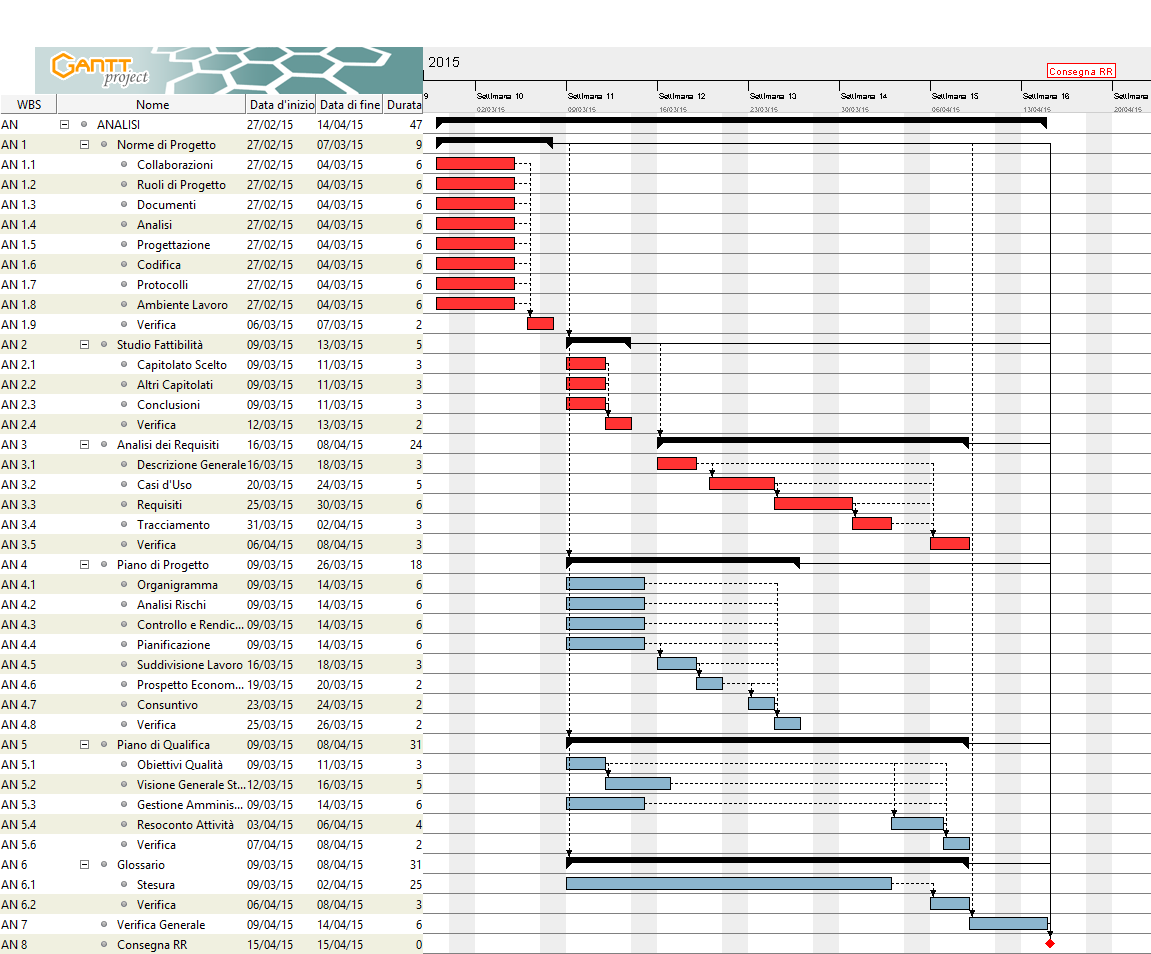
\includegraphics[width=\textwidth]{./img/analisi.png}
	\caption{Diagramma di Gantt della fase di Analisi}
\end{figure}

\newpage
\subsubsection{Work Breakdown Structure fase di Analisi}

\newpage
\subsection{Analisi di Dettaglio}
\begin{description}
	\item[Periodo:] Dal 2015.04.16 al 2015.04.28 .
\end{description}
Questa macro-fase inizia subito dopo la consegna dei documenti in ingresso per la \textbf{Revisione dei Requisiti} e termina con l'inizio della fase di \textbf{Progettazione Architetturale}. Questo periodo serve a consolidare i requisiti richiesti, migliorando il documento di \textit{Analisi dei Requisiti} ed incrementando i contenuti degli altri documenti. 

\noindent I ruoli maggiormente coinvolti sono: \textit{Analista}, \textit{Amministratore di Progetto} e \textit{Responsabile di Progetto}.
\subsubsection{Diagramma di Gantt: Analisi di Dettaglio}
\begin{figure}[h]
\centering
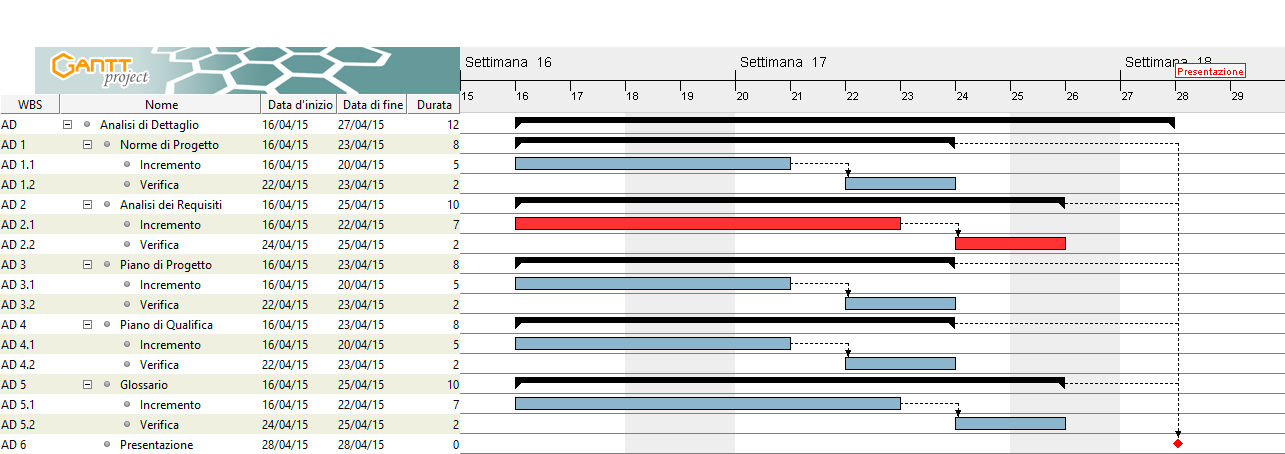
\includegraphics[width=\textwidth]{./img/analisi_dettaglio.png}
\caption{Diagramma di Gantt della fase di Analisi di Dettaglio}
\end{figure}
\newpage
\subsubsection{Work Breakdown Structure fase di Analisi di Dettaglio}

\newpage
\subsection{Progettazione Architetturale}
\begin{description}
	\item[Periodo:] Dal 2015.04.29 al 2015.05.24 .
\end{description}
Questa macro-fase inizia al concludersi dell'\textbf{Analisi di Dettaglio} e termina con la consegna della \textbf{Revisione di Progetto}. 

\noindent Le macro-attività principali di questa fase sono:
\begin{itemize}
	\item \textbf{Specifica Tecnica:} il \textit{Progettista} espone le scelte progettuali ad alto livello che si intendono inserire nel prodotto che si andrà a sviluppare.	Verranno descritti anche i Design Pattern utilizzati nella creazione del prodotto, l'architettura generale del software, i principali flussi di controllo ed il tracciamento dei requisiti;
	\item \textbf{Incremento e Verifica:} verranno aggiornati ed incrementati tutti i documenti redatti sino ad ora in base ai risultati della \textit{Revisione dei Requisiti}.	
\end{itemize}
I ruoli maggiormente coinvolti in questa macro-fase sono: \textit{Analista}, \textit{Progettista}, \textit{Verificatore}. 
\subsubsection{Diagramma di Gantt: Progettazione Architetturale}
\begin{figure}[h] 
	\centering
	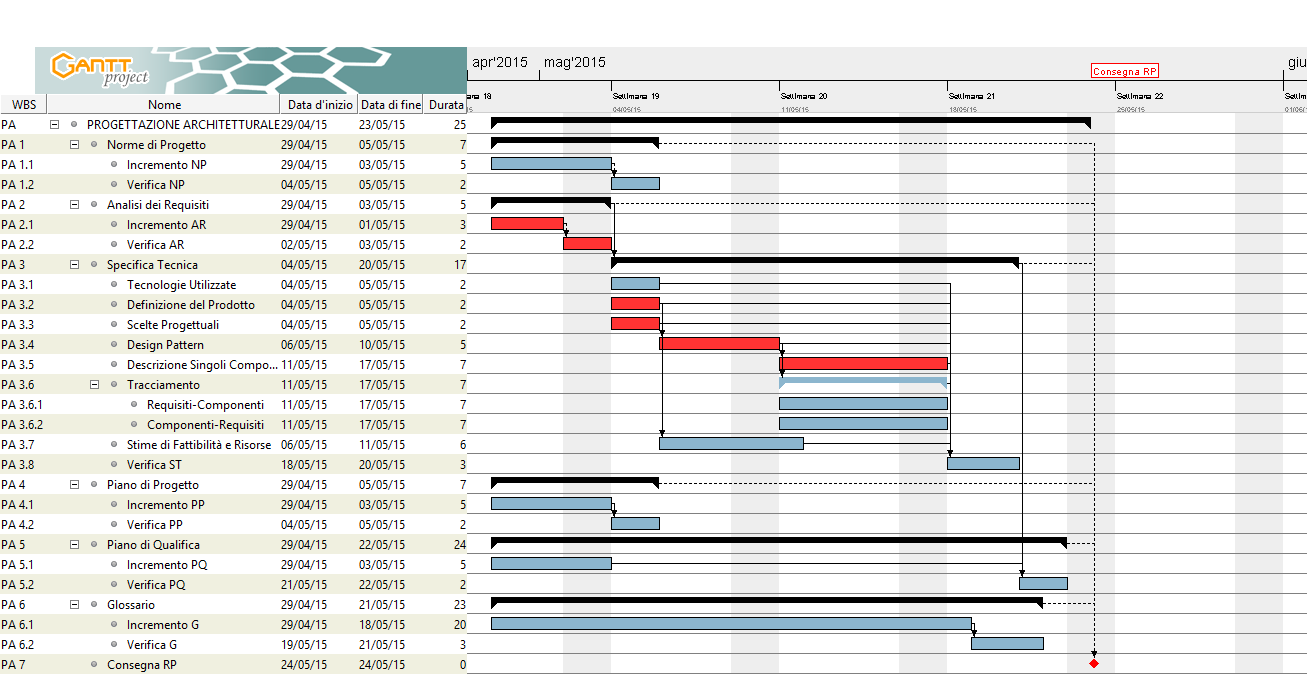
\includegraphics[width=\textwidth]{./img/progettazione_architetturale.png}
	\caption{Diagramma di Gantt della fase di Progettazione Architetturale}
\end{figure}
\newpage
\subsubsection{Work Breakdown Structure fase di Progettazione Architetturale}

\newpage
\subsection{Progettazione di Dettaglio e Codifica}
\begin{description}
	\item[Periodo:] Dal 2015.05.30 al 2015.06.13 .
\end{description}
Questa macro-fase ha inizio con la consegna della \textbf{Revisione di Progetto} e termina con la consegna della \textbf{Revisione di Qualifica}. 

\noindent Le macro-attività principali di questa fase sono:
\begin{itemize}
	\item \textbf{Definizione di Prodotto:} vengono definite in maniera più approfondita la struttura e le relazioni delle componenti del prodotto, sulla base del documento di \textit{Specifica Tecnica};
	\item \textbf{Codifica:} seguendo quanto scritto nella \textit{Definizione di Prodotto}, i programmatori iniziano a sviluppare il codice del programma. Questa macro-attività è stata suddivisa in due attività, in quanto, adottando un ciclo di vita incrementale, nel primo ciclo verranno realizzate le parti che riguardano i requisiti obbligatori mentre nel secondo verrà valutato, in base al tempo disponibile e all'interesse del gruppo, la possibilità di sviluppare funzionalità aggiuntive opzionali e desiderabili da inserire nel prodotto;
	\item \textbf{Manuali Utente:} verranno redatti una volta finito lo sviluppo del codice e avranno lo scopo di fornire delle linee guida per l'utilizzo del sistema da parte degli utenti coinvolti;
	\item \textbf{Incremento e Verifica:} verranno aggiornati ed incrementati tutti i documenti redatti sino ad ora in base ai risultati della \textit{Revisione di Progettazione}.
\end{itemize}
I ruoli più utilizzati in questa macro-fase sono: \textit{Progettista}, \textit{Programmatore} e \textit{Verificatore}. 
\subsubsection{Diagramma di Gantt: Progettazione di Dettaglio}
\begin{figure}[h] 
	\centering
	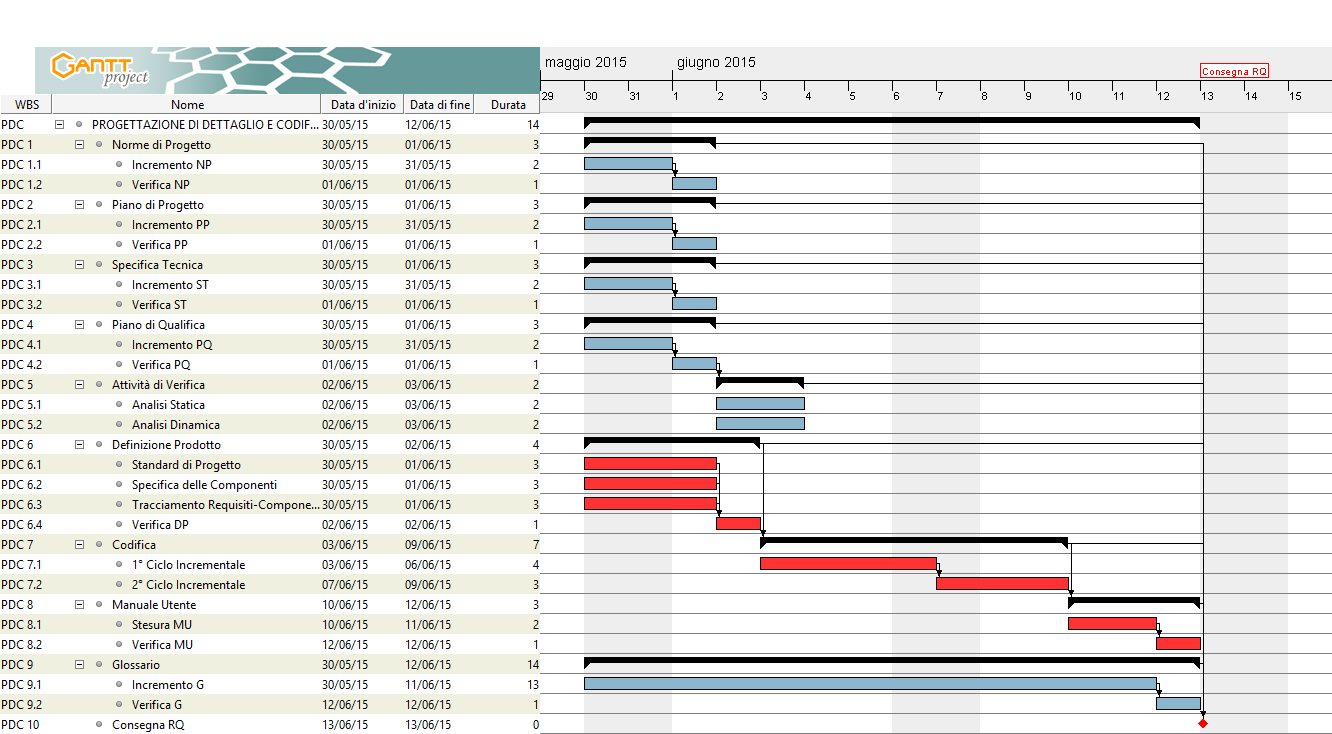
\includegraphics[width=\textwidth]{./img/progettazione_dettaglio.png}
	\caption{Diagramma di Gantt della fase di Progettazione di Dettaglio}
\end{figure}
\newpage
\subsubsection{Work Breakdown Structure fase di Progettazione di Dettaglio}

\newpage
\subsection{Verifica e Validazione}
\begin{description}
	\item[Periodo:] Dal 2015.06.19 al 2015.07.03 .
\end{description}
Questa macro-fase ha inizio alla consegna della \textbf{Revisione di Qualifica} e ha termine con la consegna della \textbf{Revisione di Accettazione}, cioè col termine del processo dello sviluppo del software.

\noindent Le macro-attività principali di questa fase sono:
\begin{itemize}
	\item \textbf{Validazione Verifica e Collaudo del Sistema:} il prodotto verrà convalidato per testare che è conforme alle specifiche e che soddisfa le richieste espresse dal cliente nel capitolato;
	\item \textbf{Incremento e Verifica:} verranno aggiornati ed incrementati tutti i documenti redatti sino ad ora in base ai risultati della \textit{Revisione di Qualifica}.
\end{itemize}
Si noti che non è da intendersi che le verifiche necessarie vengano fatte solamente durante la macro-fase di \textbf{Verifica e Validazione}. Tale macro-fase incorpora le attività necessarie per il collaudo del prodotto. La verifica è un'attività presente in tutte le macro-fasi precedenti e non è dunque da confondere con questa macro-fase.

\noindent I ruoli più utilizzati in questa macro-fase sono: \textit{Progettista}, \textit{Programmatore} e \textit{Verificatore}.
\subsubsection{Diagramma di Gantt: Verifica e Validazione}
\begin{figure}[h] 
	\centering
	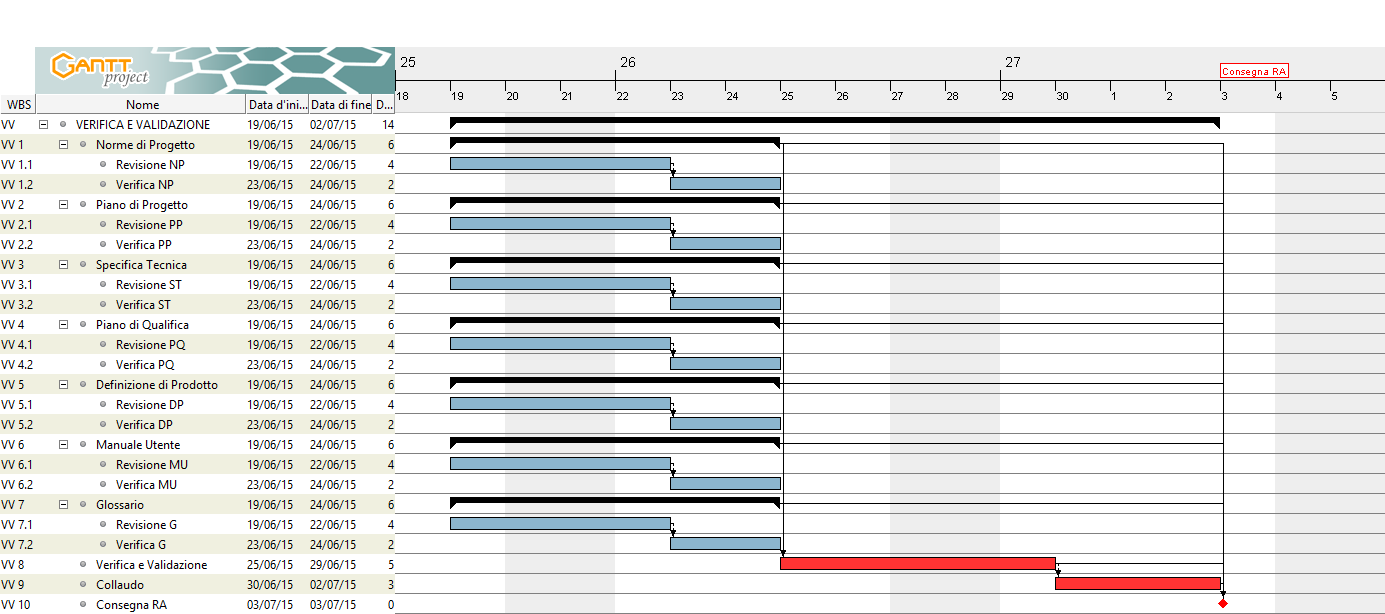
\includegraphics[width=\textwidth]{./img/verifica_validazione.png}
	\caption{Diagramma di Gantt della fase di Verifica e Validazione}
\end{figure}
\newpage
\subsubsection{Work Breakdown Structure fase di Verifica e Validazione}
